

\tikzset{every picture/.style={line width=0.75pt}} %set default line width to 0.75pt        

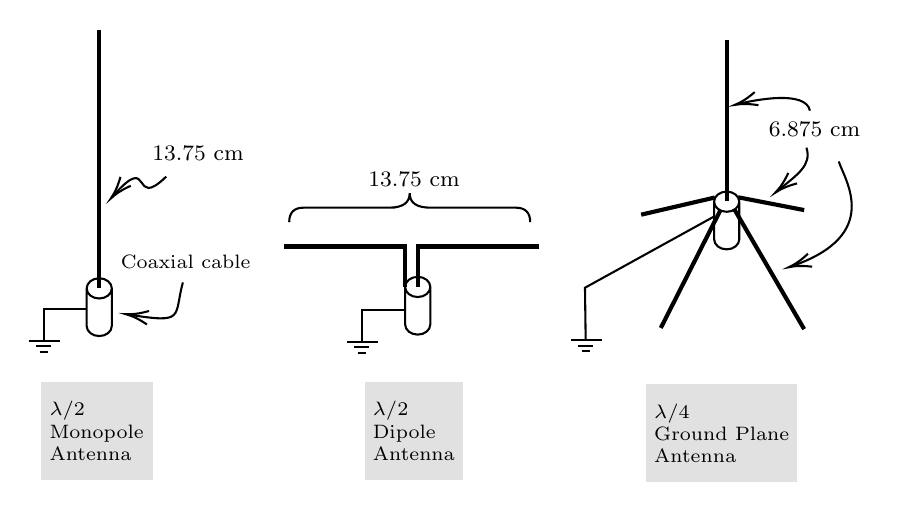
\begin{tikzpicture}[x=0.75pt,y=0.75pt,yscale=-1,xscale=1]
%uncomment if require: \path (0,285); %set diagram left start at 0, and has height of 285

%Flowchart: Magnetic Disk [id:dp9203753850829601] 
\draw   (73.36,147.61) -- (73.36,165.71) .. controls (73.36,168.4) and (70.65,170.58) .. (67.3,170.58) .. controls (63.96,170.58) and (61.25,168.4) .. (61.25,165.71) -- (61.25,147.61)(73.36,147.61) .. controls (73.36,150.3) and (70.65,152.48) .. (67.3,152.48) .. controls (63.96,152.48) and (61.25,150.3) .. (61.25,147.61) .. controls (61.25,144.92) and (63.96,142.73) .. (67.3,142.73) .. controls (70.65,142.73) and (73.36,144.92) .. (73.36,147.61) -- cycle ;
%Straight Lines [id:da34747813628770396] 
\draw [line width=1.5]    (67.3,23) -- (67.3,147.19) ;
%Flowchart: Magnetic Disk [id:dp8472157603764505] 
\draw   (375.67,105.84) -- (375.67,123.94) .. controls (375.67,126.63) and (372.96,128.81) .. (369.61,128.81) .. controls (366.27,128.81) and (363.56,126.63) .. (363.56,123.94) -- (363.56,105.84)(375.67,105.84) .. controls (375.67,108.53) and (372.96,110.71) .. (369.61,110.71) .. controls (366.27,110.71) and (363.56,108.53) .. (363.56,105.84) .. controls (363.56,103.15) and (366.27,100.97) .. (369.61,100.97) .. controls (372.96,100.97) and (375.67,103.15) .. (375.67,105.84) -- cycle ;
%Straight Lines [id:da5662262777033016] 
\draw [line width=1.5]    (369.61,28.01) -- (369.61,105.42) ;
%Straight Lines [id:da13460916170815418] 
\draw [line width=1.5]    (363.9,103.83) -- (328.4,112.1) ;
%Straight Lines [id:da574222375987339] 
\draw [line width=1.5]    (406.93,167.24) -- (373.44,109.74) ;
%Straight Lines [id:da3064624130741478] 
\draw [line width=1.5]    (337.87,166.68) -- (366.5,110.1) ;
%Straight Lines [id:da5811958206568459] 
\draw [line width=1.5]    (406.93,109.88) -- (375.11,103.72) ;
%Curve Lines [id:da621153715774825] 
\draw    (409.71,61.98) .. controls (407.71,51.96) and (383.15,56.82) .. (375.41,58.71) ;
\draw [shift={(373.51,59.2)}, rotate = 344.05] [color={rgb, 255:red, 0; green, 0; blue, 0 }  ][line width=0.75]    (10.93,-3.29) .. controls (6.95,-1.4) and (3.31,-0.3) .. (0,0) .. controls (3.31,0.3) and (6.95,1.4) .. (10.93,3.29)   ;
%Curve Lines [id:da20820331798614888] 
\draw    (408.04,79.8) .. controls (410.69,88.27) and (403.78,92.71) .. (394.49,100.3) ;
\draw [shift={(393,101.52)}, rotate = 320.19] [color={rgb, 255:red, 0; green, 0; blue, 0 }  ][line width=0.75]    (10.93,-3.29) .. controls (6.95,-1.4) and (3.31,-0.3) .. (0,0) .. controls (3.31,0.3) and (6.95,1.4) .. (10.93,3.29)   ;
%Curve Lines [id:da7479713733277822] 
\draw    (99.6,93.73) .. controls (82.14,110.65) and (93.56,81.03) .. (74.1,102.9) ;
\draw [shift={(72.87,104.31)}, rotate = 310.82] [color={rgb, 255:red, 0; green, 0; blue, 0 }  ][line width=0.75]    (10.93,-3.29) .. controls (6.95,-1.4) and (3.31,-0.3) .. (0,0) .. controls (3.31,0.3) and (6.95,1.4) .. (10.93,3.29)   ;
%Straight Lines [id:da9730091494366713] 
\draw    (33.33,172.81) -- (48.37,172.81) ;
%Straight Lines [id:da05895285604419476] 
\draw    (36.9,175.59) -- (44.14,175.59) ;
%Straight Lines [id:da324980097446699] 
\draw    (38.57,178.15) -- (42.47,178.15) ;

%Straight Lines [id:da3818709999372871] 
\draw    (40.57,172.7) -- (40.57,157.66) -- (61.29,157.66) ;
%Straight Lines [id:da4499961816622231] 
\draw    (294.52,172.39) -- (309.55,172.39) ;
%Straight Lines [id:da6922155263599932] 
\draw    (298.08,175.17) -- (305.32,175.17) ;
%Straight Lines [id:da4456696138094858] 
\draw    (299.75,177.74) -- (303.65,177.74) ;

%Straight Lines [id:da16679558461507527] 
\draw    (301.67,172.32) -- (301.34,147.3) -- (363.49,113.01) ;
%Straight Lines [id:da7355318584367416] 
\draw [line width=1.5]    (279.28,127.42) -- (220.81,127.42) -- (220.81,146.91) ;
%Straight Lines [id:da25011934904681166] 
\draw [line width=1.5]    (156.23,127.42) -- (214.7,127.42) -- (214.7,146.91) ;
%Flowchart: Magnetic Disk [id:dp2241547095005254] 
\draw   (226.81,146.91) -- (226.81,165.01) .. controls (226.81,167.7) and (224.1,169.88) .. (220.75,169.88) .. controls (217.41,169.88) and (214.7,167.7) .. (214.7,165.01) -- (214.7,146.91)(226.81,146.91) .. controls (226.81,149.6) and (224.1,151.78) .. (220.75,151.78) .. controls (217.41,151.78) and (214.7,149.6) .. (214.7,146.91) .. controls (214.7,144.22) and (217.41,142.04) .. (220.75,142.04) .. controls (224.1,142.04) and (226.81,144.22) .. (226.81,146.91) -- cycle ;
%Straight Lines [id:da19895333176103813] 
\draw    (186.57,173.22) -- (201.61,173.22) ;
%Straight Lines [id:da8931773949500925] 
\draw    (190.14,176.01) -- (197.38,176.01) ;
%Straight Lines [id:da22035216453021045] 
\draw    (191.81,178.57) -- (195.71,178.57) ;

%Straight Lines [id:da35718244675007793] 
\draw    (193.81,173.11) -- (193.81,158.08) -- (214.53,158.08) ;
%Shape: Brace [id:dp32284987028621814] 
\draw   (274.94,115.72) .. controls (274.94,111.05) and (272.61,108.72) .. (267.94,108.72) -- (226.88,108.72) .. controls (220.21,108.72) and (216.88,106.39) .. (216.88,101.72) .. controls (216.88,106.39) and (213.55,108.72) .. (206.88,108.72)(209.88,108.72) -- (165.83,108.72) .. controls (161.16,108.72) and (158.83,111.05) .. (158.83,115.72) ;
%Curve Lines [id:da030068990122400274] 
\draw    (423.63,86.49) .. controls (426.39,95.31) and (444.98,121.87) .. (400.77,136.99) ;
\draw [shift={(399.41,137.44)}, rotate = 341.88] [color={rgb, 255:red, 0; green, 0; blue, 0 }  ][line width=0.75]    (10.93,-3.29) .. controls (6.95,-1.4) and (3.31,-0.3) .. (0,0) .. controls (3.31,0.3) and (6.95,1.4) .. (10.93,3.29)   ;
%Curve Lines [id:da013796374008901102] 
\draw    (107.6,144.73) .. controls (103.09,161.65) and (108.89,164.58) .. (81.71,160.27) ;
\draw [shift={(80,160)}, rotate = 369.15] [color={rgb, 255:red, 0; green, 0; blue, 0 }  ][line width=0.75]    (10.93,-3.29) .. controls (6.95,-1.4) and (3.31,-0.3) .. (0,0) .. controls (3.31,0.3) and (6.95,1.4) .. (10.93,3.29)   ;

% Text Node
\draw (114.92,82.59) node  [font=\footnotesize] [align=left] {13.75 cm};
% Text Node
\draw (411.94,70.89) node  [font=\footnotesize] [align=left] {6.875 cm};
% Text Node
\draw  [draw opacity=0][fill={rgb, 255:red, 225; green, 225; blue, 225 }  ,fill opacity=1 ]  (39.04,192.73) -- (93.04,192.73) -- (93.04,239.73) -- (39.04,239.73) -- cycle  ;
\draw (66.04,216.23) node  [font=\scriptsize] [align=left] {$\displaystyle \lambda /2\ $\\Monopole\\Antenna};
% Text Node
\draw  [draw opacity=0][fill={rgb, 255:red, 225; green, 225; blue, 225 }  ,fill opacity=1 ]  (330.72,193.73) -- (403.72,193.73) -- (403.72,240.73) -- (330.72,240.73) -- cycle  ;
\draw (367.22,217.23) node  [font=\scriptsize] [align=left] {$\displaystyle \lambda /4\ $\\Ground Plane\\Antenna};
% Text Node
\draw (218.97,95.12) node  [font=\footnotesize] [align=left] {13.75 cm};
% Text Node
\draw  [draw opacity=0][fill={rgb, 255:red, 225; green, 225; blue, 225 }  ,fill opacity=1 ]  (195.36,192.73) -- (242.36,192.73) -- (242.36,239.73) -- (195.36,239.73) -- cycle  ;
\draw (218.86,216.23) node  [font=\scriptsize] [align=left] {$\displaystyle \lambda /2\ $\\Dipole\\Antenna};
% Text Node
\draw (108.92,134.59) node  [font=\scriptsize] [align=left] {Coaxial cable};


\end{tikzpicture}
